% By zmienic jezyk na angielski/polski, dodaj opcje do klasy english lub polish
\documentclass[polish,11pt]{aghthesis}
\usepackage[utf8]{inputenc}
\usepackage{url}
\usepackage{amsfonts}
\usepackage{caption}
\usepackage{enumitem}

% dodatkowe pakiety
\usepackage[hidelinks]{hyperref}

\author{Tomasz Kasprzyk, Daniel Ogiela\\ Jakub Stępak}

\title{System obliczający wyniki wyborów dla uogólnienia systemu k-Borda}

\supervisor{dr hab.\ inż.\ Piotr Faliszewski}

\date{2016}

% Szablon przystosowany jest do druku dwustronnego, 
\begin{document}

\maketitle
\tableofcontents
\clearpage

%--------------------------Rozdział Wizja produktu -----------------------------------------
%-------------------------------------------------------------------------------------------

\section{Wizja produktu}

%--------------------------Podrozdział Opis problemu ---------------------------------------
\subsection{Opis problemu}
Projekt dotyczy obliczania wyników wyborów. Wybory i sposób wyłaniania zwycięzców są
ściśle określone. Wybory można opisać jako parę $(C, V)$, gdzie $C = \left\{c_1, c_2, ... , c_m\right\}$ stanowi zbiór kandydatów, a $V = \left\{v_1, v_2, ... , v_n\right\}$ to ciąg wyborców. Każdy z wyborców posiada swoje preferencje wyborcze, które są opisane przez ciąg kandydatów ze zbioru $C$. Długość ciągu kandydatów wynosi $m$, a kandydaci są uporządkowani od najbardziej preferowanego do najmniej preferowanego. Ponadto określony jest rozmiar $k$ zwycięskiego komitetu, który określa liczbę kandydatów, którzy zwyciężyli w wyborach.
%\vspace{5mm}

\begin{center}
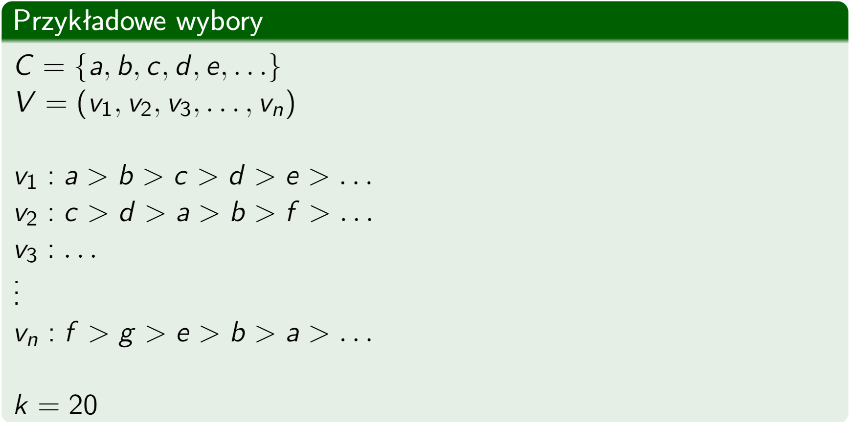
\includegraphics[width=0.8\textwidth]{pics/przykladowe_wybory.png}
\end{center}
Ciąg kandydatów przyporządkowany danemu wyborcy traktowany jest jako głos w
wyborach. Każdemu kandydatowi w ciągu stanowiącym głos, przyporządkowane są punkty
według punktacji Bordy. Jeżeli przez $i$ zostanie oznaczona pozycja danego kandydata w
ciągu stanowiącym głos (jeżeli kandydat jest pierwszy w ciągu, wtedy $i = 1$, jeśli drugi, wtedy $i = 2$ itd.), to wartość punktowa przyporządkowana według metody Bordy w tym głosie dla tego kandydata wynosi $\beta(i) = m - i$ , gdzie $m$ to rozmiar zbioru $C$ (liczba wszystkich kandydatów). Zatem dla danego głosu kolejni uporządkowani kandydaci otrzymują kolejno $m - 1, m - 2, … , 1, 0$ punktów.

\begin{center}

\includegraphics[width=0.8\textwidth]{pics/Borda_points.png}
\end{center}
W celu wyłonienia zwycięzców wyborów komitetów definiuje się tzw. funkcję satysfakcji,
która bazuje między innymi na punktacji metodą Bordy. Funkcja satysfakcji określa
zadowolenie danego wyborcy ze zwycięskiego komitetu. W celu zwięzłego zdefiniowania
funkcji celu wprowadza się pojęcie ciągu pozycji, które określa dla danego wyborcy pozycje
wszystkich zwycięskich kandydatów z jego preferencji. Ciąg pozycji jest posortowany
rosnąco - pozycja najbardziej preferowanego kandydata spośród zwycięzców na początku
ciągu, pozycja najmniej preferowanego kandydata spośród zwycięzców na końcu ciągu.
\clearpage
\noindent
\emph{Przykład} \\ 
Dla następujących preferencji:
\begin{center}

\includegraphics[width=0.8\textwidth]{pics/positions.png}
\end{center}
komitetu $K = \left\{a, b, e\right\}$ i wyborcy $v_3$ ciąg pozycji oznaczany ${pos_v}_3$ wynosi $(3,4,6)$, gdyż pozycja najlepszego kandydata ze zbioru $K$ wynosi $3$ (kandydat $e$), druga najlepsza to pozycja nr $4$ (kandydat $b$), a ostatnią pozycją najmniej preferowanego kandydata jest pozycja nr $6$ (kandydat $a$). \\ \\
W tym momencie można zdefiniować funkcję satysfakcji, która jako argument przyjmuje
zdefiniowany przed chwilą ciąg pozycji, który dla każdego wyborcy $i$ dla każdego komitetu
jest określony jednoznacznie. Funkcja satysfakcji określająca zadowolenie danego wyborcy
ze zwycięskiego komitetu, będzie więc oznaczana jako $f(i_1, i_2, ... , i_k)$. \\ \\
Poprzez różne zdefiniowanie funkcji satysfakcji, definiowane są odmienne systemy
wyborcze. Znanymi systemami wyborczymi są system $k-Borda$ oraz system
$Chamberlin-Courant’a$. Funkcje satysfakcji dla tych systemów określone są odpowiednio:
$$f_{k-Borda}(i_1, i_2, ..., i_k) = \beta(i_1) + \beta(i_2) + ... + \beta(i_k) 
$$ $$f_{CC}(i_1, i_2, ..., i_k) = \beta(i_1) = max(\beta(i_1), \beta(i_2), ..., \beta(i_k))$$
Wyniki wyborów dla podanych systemów mogą być różne (i zazwyczaj są) pomimo takich
samych danych wejściowych. Inaczej rzecz ujmując, zwycięskie komitety mogą składać się z
różnych kandydatów po zastosowaniu odmiennych funkcji satysfakcji. \\ \\
Funkcja satysfakcji, która dotyczy niniejszego projektu inżynierskiego jest oparta na normie
$\ell_p$ . Norma $\ell_p$ zdefiniowana jest następująco:
$$\ell_p(x_1,x_2,\dots, x_n) = \sqrt[p]{x_1^p+x_2^p+\dots+x_n^p}$$
, gdzie $x_1, x_2, ..., x_n \in \mathbb{R}, p \in \mathbb{N}$ \\ \\
Dla skrajnych przypadków, gdy $p = 1$ i gdy $p \to \infty$ norma $\ell_p$ przyjmuje odpowiednio postać sumy: $$l_1(x_1, x_2,\dots, x_n) = x_1 + x_2 +\dots+ x_n$$ oraz postać operatora maksimum: $$l_\infty(x_1, x_2,\dots, x_n) = max(x_1, x_2,\dots, x_n)$$
\\ Mając zdefiniowaną normę $\ell_p$ można określić funkcję satysfakcji będącą tematem pracy. $$f_{{\ell_p}-Borda}(i_1, i_2, ..., i_k) = \ell_p(\beta(i_1), \beta(i_2), ..., \beta(i_k)) = \sqrt[p]{[\beta(i_1)]^p+[\beta(i_2)]^p+\dots+[\beta(i_k)]^p}$$
\clearpage
Funkcja jest uogólnieniem systemu $k-Borda$. Jeżeli za $p$ przyjęta zostanie wartość $1$,
zdefiniowana funkcja przyjmuje postać funkcji satysfakcji dla zwykłego systemu $k-Borda$. Dla $p$ dążącego do nieskończoności funkcja przyjmuje postać funkcji satysfakcji dla systemu
$Chamberlin-Courant’a$.

% ------------------------------------------------------------------------------------------

%--------------------------Podrozdział Możliwości ------------------------------------------
\subsection{Możliwości}
Obliczanie wyników wyborów dla systemu $\ell_p-Borda$ metodą typu brute-force jest
czasochłonne. Już dla stosunkowo niewielkich rozmiarem danych, algorytm jest nieużyteczny. Dlatego głównym zadaniem projektu jest zaprojektowanie i implementacja algorytmów heurystycznych, które możliwie dokładnie i możliwie szybko obliczają wyniki wyborów. Ponadto do zadań zespołu należy próba oceny działania stworzonych algorytmów heurystycznych.

% ------------------------------------------------------------------------------------------

%--------------------------Motywacja do stworzenia projektu --------------------------------
\subsection{Motywacja do stworzenia projektu}
Jednym z głównym celów realizacji projektu jest chęć poznania różnych sposobów tworzenia
algorytmów heurystycznych oraz zastosowanie ich do rozwiązania problemów w
interesującej zespół tematyce, jaką jest sposób wyłaniania zwycięzców w wyborach i
związek między tym sposobem a satysfakcją wyborców ze zwycięzców. Ponadto zespół
chciał porównać pod różnymi względami różne algorytmy heurystyczne. Interesujące jest
zestawienie algorytmów pod względem dokładności obliczanych rozwiązań, czasu działania,
czy trudności w projektowaniu i implementacji. 

Drugą, istotną motywacją do stworzenia systemu jest możliwość wykorzystania go do wielu
bardzo różnych sytuacji. Zdefiniowanie wyborów, których wyniki ma liczyć system, może
dotyczyć różnego rodzaju wyborów. Mogą to być wybory ludzi do wszelakiego typu organów
władz na różnych szczeblach organizacji państwowych lub organizacji prywatnych. Wybory
nie muszą dotyczyć ludzi, a mogą polegać na selekcji innych rzeczy. Można zdefiniować
wybory na filmy, które zostaną odtworzone w trakcie podróży samolotem, czy podczas
seansu z rodziną i znajomymi. Mogą to być wybory na miejsca wspólnego wypadu znajomych na weekend. Wszędzie, gdzie ma sens zastosowanie preferencji (ułożenie
rzeczy od najbardziej do najmniej pożądanej) można wykorzystać stworzony system.

Dzięki stworzonemu systemowi według określonych wymagań, możliwe jest nie tylko
szybkie obliczenie wyborów na bazie wprowadzonych do systemu preferencji. Możliwe jest
sterowaniem sposobem obliczania wyborów według pożądanej reprezentatywności
zwycięskich kandydatów. Można decydować czy zwycięzcy wyborów będą tacy, że każdy
znajdzie wśród nich takiego, którego bardzo lubi, ale też taki, którego bardzo nie lubi. Czy
może zwycięzcy mają być tacy, że większość wyborców co prawda nie znajdzie wśród nich
bardzo pożądanego kandydata, ale jednocześnie nie znajdzie takiego, którego bardzo nie
lubi. Możliwy jest również wybór pośredni między wskazanymi dwoma rozwiązaniami.

Przykładowo, jeżeli użytkownik chce wybrać kilka filmów do wspólnego seansu z
przyjaciółmi i rodziną, to może zdecydować między różnymi opcjami. Jedną z opcji jest taki
wybór, aby wśród wybranych filmów każdy ze znajomych znalazł film, który mu bardzo
odpowiada, lecz jednocześnie znalazły się takie, które większości znajomych wyraźnie nie
odpowiadają. Druga możliwość to taka, w której wybrane zostaną filmy, które większości
znajomych ani za bardzo nie odpowiadają, ani za bardzo nie przeszkadzają. Pozostałymi
możliwościami są opcje pośrednie między wskazanymi.
\clearpage

% ------------------------------------------------------------------------------------------

%--------------------------Podrozdział Użytkownicy -----------------------------------------
\subsection{Użytkownicy}
Potencjalnymi użytkownikami systemu mogą być osoby i organizacje, które potrzebują
systemu wybierania kilku elementów spośród puli wszystkich elementów w taki sposób, aby
usatysfakcjonować swoich klientów. System może mieć przykładowe zastosowanie dla
przedsiębiorstw realizujących usługi transportu lotniczego czy autokarowego do umilenia
czasu podróży poprzez wybór odpowiednich filmów czy potraw. Ponadto system może
służyć pojedynczym osobom w celu wyboru odpowiedniej formy spędzania wolnego czasu w
grupie znajomych.

% ------------------------------------------------------------------------------------------

%--------------------------Podrozdział Usługi dostarczane przez system ---------------------
\subsection{Usługi dostarczanie przez system}

\subsubsection{Usługi wymagane}
\begin{itemize}
    \item możliwość wprowadzenia wyborów do systemu
    \item obliczenie wyników wyborów
    \item wyświetlanie wyników wyborów
\end{itemize}

\subsubsection{Usługi pożądane}
\begin{itemize}
    \item możliwość zarządzania swoimi wyborami (dodawanie nowych wyborów, nowych wyników, porównywanie różnych rezultatów)
    \item intuicyjna nawigacja po systemie
\end{itemize}

\subsubsection{Usługi dodatkowe}
\begin{itemize}
    \item wygodny sposób definiowania wyborów - zadanie projektowe koncentruje się na
projektowaniu i tworzeniu algorytmów obliczających wyniki wyborów. System musi
wczytywać pewien format pliku wejściowego definiującego wybory, który niekoniecznie jest prosty i intuicyjny w tworzeniu. Jeżeli ta dodatkowa usługa zostałaby zrealizowana, ułatwiłaby użytkowanie systemu i poprawiła zadowolenie użytkowników z korzystania z systemu
\end{itemize}

% ------------------------------------------------------------------------------------------

%-------------------------------------------------------------------------------------------
%-------------------------------------------------------------------------------------------
\section{Studium wykonalności}
  
\subsection{Opis wymagań}

\subsubsection{Wymagania funkcjonalne}
Poniżej zamieszczona jest lista najważniejszych wymagań w postaci kolejnych tabel. Tabela składa się z trzech pól opisujących dane wymaganie: \textit{Nazwa, Opis} i \textit{Uzasadnienie}. Pole \textit{Nazwa} jest nazwą usługi dostarczanej przez system, pole \textit{Opis} szczegółowo opisuje w jaki sposób jest realizowane dane wymaganie, a pole \textit{Uzasadnienie} podaje powód dlaczego w taki, a nie inny sposób wymaganie zostało zrealizowane i postawione.
\newpage
\begin{table}
\centering
\begin{tabular}{|c|p{12.5cm}|}
\hline
\textbf{Nazwa} & Zdefiniowanie wyborów \\ 
\hline 
\textbf{Opis} & System oferuje różne sposoby zdefiniowania i wprowadzenia wyborów
do systemu. Pierwszym i podstawowym jest możliwość określania
wyborów w pliku formatu $.soc$. Sposób określania w nim kandydatów
oraz głosów wyborców jest ściśle określony. W pierwszej linii pliku
znajduje się liczba kandydatów do zwycięskiego komitetu. W kolejnych
liniach znajdują się numery i nazwy kandydatów. Następnie jest linia z
informacją o liczbie głosujących, liczbie policzonych głosów oraz liczbie
głosów unikalnych. W ostatnim bloku pliku znajdują się linie z
informacją o preferencjach głosów unikalnych. Każda linia składa się z
liczby powtórzeń danego głosu oraz preferencji określonej dla tego
głosu, która ma postać ciągu numerów kandydatów od najbardziej do
najmniej pożądanego. Po stworzeniu opisanego pliku system umożliwia
wskazanie pliku z systemu plików.

Drugim sposobem definiowania wyborów oferowanym przez system
jest generowanie wyborów z rozkładu normalnego. W tym celu
kandydaci i wyborcy są reprezentowani jako punkty płaszczyźnie.
Preferencje wyborców obliczane są na bazie odległości euklidesowych
do poszczególnych kandydatów na płaszczyźnie. Aby wygenerować
wybory użytkownik podaje w formularzu parametry potrzebne do
generacji wyborów zgodnie z rozkładem normalnym. Uzupełnia pola
dotyczące: liczby kandydatów, średniej wartości współrzędnej $x$ dla
wyborców, średniej wartości współrzędnej x dla kandydatów, średniej
wartości współrzędnej $y$ dla wyborców, średniej wartości współrzędnej
$y$ dla kandydatów, odchylenia standardowego wyborców oraz
odchylenia standardowego kandydatów. \\ 
\hline 
\textbf{Uzasadnienie} & Definicja wyborów za pomocą pliku formatu $.soc$ zapewnia spełnienie
podstawowej usługi oferowanej przez system - wprowadzenia wyborów
do systemu. Uzasadnieniem dla konieczności generacji wyborów z
rozkładu normalnego jest możliwość atrakcyjnej i klarownej wizualizacji
wyborów i wyników wyborów. Wizualizacja w ten sposób wyników
wyborów umożliwia między innymi ocenienie jakości stworzonych
algorytmów i porównanie ich.\\ 
\hline 
\end{tabular}
\caption{Zdefiniowanie wyborów} 
\end{table}

\begin{table}
\centering
\begin{tabular}{|c|p{10cm}|}
\hline
\textbf{Nazwa} & Obliczanie wyników wyborów \\ 
\hline 
\textbf{Opis} & System oferuje kilka algorytmów heurystycznych obliczających wyniki
wyborów. Algorytmy bazują na różnym paradygmacie tworzenia ich.
Jeden z paradygmatów to programowanie zachłanne, a drugi to
programowanie genetyczne. Algorytmy dają przybliżone rozwiązania
problemu pod względem jego dokładności. Użytkownik przy tworzeniu
nowego wyniku dla zdefiniowanych wyborów może w prosty sposób
wybrać jeden z algorytmów. \\ 
\hline 
\textbf{Uzasadnienie} & Kilka stworzonych algorytmów i różne podejście do tworzenia ich,
umożliwia ocenę jakości algorytmów na bazie zestawienia wyników
obliczonych wyborów. Ponadto stworzenie różnych algorytmów pozwoli
na dogłębniejsze poznanie sposobów tworzenia algorytmów
heurystycznych, jak również samej tematyki pracy, jaką były różne
sposoby wyboru zwycięskiego komitetu.\\ 
\hline 
\end{tabular}
\caption{Obliczanie wyników wyborów} 
\end{table}
\clearpage

%\begin{table}
{
\centering
\begin{tabular}{|c|p{10cm}|}
\hline
\textbf{Nazwa} & Wersja algorytmu zachłannego $Greedy - CC$ \\ 
\hline 
\textbf{Opis} & Implementacja algorytmu zachłannego dla szczególnego przypadku
(parametr $p \to \infty$) \\ 
\hline 
\textbf{Uzasadnienie} & Dla stosunkowo "dużych" wartości parametru $p$ wykonywanie operacji
pierwiastkowania i potęgowania stanowi niepotrzebny narzut czasowy.
W tym przypadku operację obliczania normy $\ell_p$ można zastąpić
wyznaczaniem maksimum dla pojedynczych wyników kandydatów z
komitetu, dla którego liczono by normę $\ell_p$.
Korzyści jakie płyną z takiej modyfikacji to nie tylko skrócenie czasu
obliczeń, ale także ustalanie od jakiej wartości parametru $p$ komitet
wygrywający jest zgodny z wynikiem otrzymanym dla systemu
$Chamberlin-Courant’a$.\\ 
\hline 
\end{tabular} 
\captionof{table}{Wersja algorytmu zachłannego $Greedy - CC$}
}
%\end{table}
\vspace{\baselineskip}
%\begin{table}
{
\centering
\begin{tabular}{|c|p{10cm}|}
\hline
\textbf{Nazwa} & Prezentacja wyników wyborów \\ 
\hline 
\textbf{Opis} & System oferuje dwa sposoby prezentacji wyników wyborów. Pierwszy z
nich, to proste wskazanie kandydatów i wypisanie nazw kandydatów w
widocznym panelu. Ta forma prezentacji dotyczy wyników wyborów,
które zdefiniowane zostały za pomocą pliku formatu $.soc$.

Druga forma prezentacji wyników wyborów dotyczy wyborów wygenerowanych z
rozkładu normalnego. Wizualizacja polega na narysowaniu wykresu
$2D$, na którym punkty reprezentujące kandydatów ze zwycięskiego
komitetu są wyraźnie wyróżnione na tle kandydatów, którzy nie dostali
się do zwycięskiego komitetu. Dla wyborów generowanych z rozkładu normalnego system również oferuje wypisanie nazw zwycięzców w dobrze widocznym panelu.\\ 
\hline 
\textbf{Uzasadnienie} & Prezentacja wyników wyborów w postaci wykresu $2D$ z wyraźnie
zaznaczonymi zwycięzcami i przegranymi, którzy są reprezentowani
jako punkty, pozwala na porównanie w prosty sposób wyników
wyborów dla różnych wartości parametru $p$. Taka forma wizualizacji
jest jednocześnie wizualnie atrakcyjna.
Prezentacja wyników dla wyborów zdefiniowanych z pliku formatu $.soc$
ogranicza się jedynie do wypisania zwycięzców, ponieważ kandydaci
nie są reprezentowani jako punkty i tym samym nie mają
współrzędnych w tej odmianie wyborów.\\ 
\hline 
\end{tabular} 
\captionof{table}{Prezentacja wyników wyborów}
}
%\end{table}

%\clearpage
\subsubsection{Wymagania niefunkcjonalne}
Wymagania niefunkcjonalne podzielono na wymagania produktowe i wymagania organizacyjne. Poniżej zamieszczono tabele analogiczne do tych z wymagań funkcjonalnych dla odpowiednich typów wymagań niefunkcjonalnych.
\clearpage
\begin{center}
\textbf{Wymagania produktowe}
\end{center}
{
\centering
\begin{tabular}{|c|p{10cm}|}
\hline
\textbf{Nazwa} & Obliczanie wyników wyborów w satysfakcjonującym czasie \\ 
\hline 
\textbf{Opis} & Ponieważ dla już stosunkowo małych danych metoda brute-force
rozwiązywania opisanego problemu nie daje rezultatów w
satysfakcjonującym czasie, więc to wymaganie niefunkcjonalne jest
kluczowe w tym projekcie. Zastosowanie algorytmów heurystycznych
wychodzi naprzeciw temu wymaganiu. Algorytmy powinny dawać
rozwiązania w zadowalającym czasie dla możliwie dużych danych. \\ 
\hline 
\textbf{Uzasadnienie} & Czas działania algorytmu powinien się mieścić w możliwym do
zaakceptowania przedziale czasu ze względu na konieczność jego
użyteczności.\\ 
\hline 
\end{tabular}
\captionof{table}{Obliczanie wyników wyborów w satysfakcjonującym czasie}
}

\begin{center}
\textbf{Wymagania organizacyjne}
\end{center}
{
\centering
\begin{tabular}{|c|p{10cm}|}
\hline
\textbf{Nazwa} & Dotrzymanie terminów na przedstawienie poszczególnych elementów
pracy \\ 
\hline 
\textbf{Opis} & Kolejne elementy pracy, które należało przedstawiać w umówionych
terminach to: wizja produktu, studium wykonalności, prototyp oraz tuż
przed końcem projektu: produkt końcowy wraz z dokumentacją. \\ 
\hline 
\textbf{Uzasadnienie} & Terminy są dostosowane do trybu wykonywania pracy inżynierskiej,
który jest ustalany przez władze uczelni.\\ 
\hline 
\end{tabular}
\captionof{table}{Obliczanie wyników wyborów w satysfakcjonującym czasie}
}

\subsection{Strategia testowania}
Podstawowym rodzajem testów pisanych w trakcie tworzenia systemu były testy
jednostkowe. Były one dodawane na bieżąco od razu przy dodawaniu kolejnych
funkcjonalności systemu. 

Ponadto w celu zagwarantowania poprawności działania wcześniej dodanych
funkcjonalności po dodaniu nowych skorzystano z ciągłej integracji. Do tego celu
wykorzystano serwis Travis Cl skonfigurowany do repozytorium kodu. Przy każdej zmianie
kodu źródłowego w repozytorium dokonywane było automatyczne włączenie testów
jednostkowych.  

Do oceny poprawności obliczanych wyników wyborów przez stworzone algorytmu,
przeprowadzono testy porównawcze. Zestawiano wyniki wyborów obliczonych przez różne
algorytmy dla tych samych danych wejściowych. Ponadto porównywano wykresy wyników
wyborów z oczekiwanymi rezultatami.
\clearpage

\subsection{Aspekt technologiczny}
Do stworzenia systemu wykorzystano język $Python \ 2.7$. Produkt postanowiono wykonać w
postaci aplikacji webowej. Aplikację internetową oparto na frameworku pythonowym $Django \
1.9$. Do tworzenia stron internetowych użyto frameworku $Bootstrap$. Do wdrożenia systemu
wykorzystano platformę $Heroku$.

Wybrano taki stos technologiczny ze względu na doświadczenie części zespołu pracy z nim.
Wiedza na temat tych narzędzi przekonywała zespół o możliwości zrealizowania projektu w
tej technologii.

\subsection{Analiza ryzyka}
Głównym zagrożeniem dla realizacji produktu mogły być problemy ze stworzeniem
wystarczająco dobrego algorytmu heurystycznego dla opisanego problemu. Ze względu na
niewielkie doświadczenie zespołu w tej dziedzinie taka sytuacja mogła wystąpić. Głównym
zabezpieczeniem na wypadek takiego scenariusza było stosunkowo szybkie stworzenie
bazy całego systemu i możliwość wczesnego skupienia się na algorytmach heurystycznych.

Innym, dużo mniejszym zagrożeniem dla projektu mógł być brak skoordynowania prac
poszczególnych członków zespołu. Ponieważ dla członków zespołu projekt inżynierski był
tylko jednym z wielu zajęć w czasie trwania projektu, mogła wystąpić sytuacja kiedy ze
względu na natężenie innych obowiązków, dany członek zespołu nie mógłby wykonać
koniecznej pracy w odpowiednim czasie.

\section{Wybrane aspekty realizacji}
\subsection{Lista modułów}
Moduły przedstawione są w postaci przyporządkowania do modułów usług, za które w
systemie odpowiedzialny jest dany moduł. Część opisanych czynności jest wykonywana
poprzez współpracę różnych modułów.

\noindent
\begin{enumerate}[leftmargin=0.5cm]
\item Moduł administracji kont
	\begin{itemize}
	\item logowanie
	\item wylogowanie
	\item rejestracja
	\end{itemize}
\item Moduł zarządzania wyborami
	\begin{itemize}
	\item wyświetlenie listy wszystkich wyborów
	\item wyświetlenie listy wszystkich wyników dla danych wyborów
	\item stworzenie nowych wyborów
	\item stworzenie nowego wyniku
	\item usunięcie wyborów
	\item usunięcie wyniku
	\end{itemize}
\item Moduł wizualizacji wyborów i wyników wyborów
	\begin{itemize}
	\item wizualizacja wyborów wygenerowanych zgodnie z rozkładem normalnym
	\item wizualizacja wyników wyborów dla wyborów wygenerowanych zgodnie z rozkładem
normalnym
	\end{itemize}
\item Moduł generacji i wczytywania wyborów
	\begin{itemize}
	\item generacja wyborów z rozkładu normalnego
	\item wczytywanie wyborów z pliku formatu $.soc$
	\end{itemize}
\item Moduł obliczania wyników wyborów
	\begin{itemize}
	\item obliczanie wyników wyborów za pomocą różnych algorytmów
	\end{itemize}
\item Moduł URL Resolver
	\begin{itemize}
	\item przekazywanie żądań otrzymywanych przez klienta do odpowiednich modułów
	\end{itemize}
\end{enumerate}

\subsection{Diagram komunikacji}
\begin{center}
\centerline{\includegraphics[scale=0.7]{pics/Diagram_Komunikacji.png}}
\captionof{figure}{Diagram komunikacji}
\end{center}

\subsubsection{Opis diagramu}
Na diagramie oprócz przytoczonych modułów znajdują się przeglądarka internetowa oraz
baza danych. W celu wykonania swoich usług moduły współpracują z tymi dodatkowymi
komponentami diagramu. Wszystkie moduły wykorzystują wewnętrzne mechanizmy $Django$,
dlatego znajdują się wewnątrz dużego obszaru oznaczonego jako $Django$. Największym
modułem spośród wszystkich modułów jest moduł zarządzania wyborami. Współpracuje on
z innymi modułami w celu wykonania niektórych swoich zadań. Zleca on między innymi
obliczenie wyników wyborów modułowi obliczania wyników wyborów przy wykonywaniu
zadania stworzenia nowego wyniku. Najbardziej odosobnionym modułem jest moduł
administracji kont, który nie współpracuje z innymi modułami. Jedynie moduł URL Resolver
kieruje odpowiednie żądania do tego modułu i jest to jedyna komunikacja związania z
modułem administracji kont. Większość modułów w celu realizacji swoich zadań komunikuje
się z bazą danych. Dokładny opis diagramu ze ścieżkami przejść znajduje się w dokumentacji
technicznej.

\section{Organizacja pracy}
\subsection{Metodyka pracy}
Tworzenie systemu będącego realizacją tego projektu inżynierskiego można uznać za
proces ewolucyjnego tworzenia oprogramowania. Klient na początku projektu określił
wymagania w bardzo ogólny sposób. Tworzony system miał za zadanie obliczać wyniki
wyborów dla zdefiniowanego przez klienta systemu wyborczego za pomocą algorytmów
heurystycznych. W miarę postępu projektu, wymagania były precyzowane na bazie częstego
kontaktu z klientem i potrzeb rozwijanego systemu. Powstawały kolejne wersje systemu aż
do osiągnięcia systemu końcowego.

\subsection{Podział prac}
W ramach realizacji projektu przydzielano prace do poszczególnych członków zespołu.
\vspace{\baselineskip} \\
Tomasz Kasprzyk
\begin{itemize}
\item czynność1
\end{itemize}
Daniel Ogiela
\begin{itemize}
\item czynność1
\end{itemize}
Jakub Stępak
\begin{itemize}
\item czynność1
\end{itemize}

\subsection{Narzędzia do zarządzania projektem}
Do przydzielania zadań członkom zespołu i ustalania ich terminów wykorzystano aplikację
internetową $Trello$. Do przechowywania kodu źródłowego oprogramowania wykorzystano
serwis internetowy $GitHub$. W celu zdalnego kontaktowania się pomiędzy członkami zespołu
korzystano z oprogramowania $Slack$. Korzystano z aplikacji $Google Docs$ do tworzenia
roboczej wersji dokumentacji. Do przygotowywania diagramów do dokumentacji
wykorzystano aplikację $draw.io$.

\subsection{Opis kolejnych wersji systemu}
\subsubsection{Wersja 1.}
Pierwsza wersja systemu była uruchamiana z poziomu konsoli Pythona. Aplikacja
przyjmowała za argumenty parametr $p$ konieczny do obliczania normy $\ell_p$ oraz plik z
rozszerzeniem $.soc$ definiujący wybory. Aplikacja potrafiła obliczyć wyniki wyborów dla
małych danych za pomocą algorytmu typu brute-force. Pierwsza wersja systemu nie spełniała wymagań stawianych systemowi. Powstała w celu dookreślenia wymagań.

\subsubsection{Wersja 2.}
Druga wersja systemu to aplikacja webowa skonfigurowana na platformie $Heroku$. Aplikacja
posiadała funkcjonalności poprzedniej wersji systemu oraz miała dodany szereg nowych
funkcjonalności. Pozwalała na zarządzanie kontami użytkowników. Każdy użytkownik mógł
mieć swoje konto i mógł zarządzać swoimi wyborami. Miał możliwość tworzenia wyborów,
usuwania wyborów, dodawania nowych wyników wyborów czy wyświetlania zwycięzców.
Ponadto użytkownik mógł generować wybory zgodnie z rozkładem normalnym według
podanych parametrów. Dla tak stworzonych wyborów użytkownik miał możliwość wyświetlić
wykresy $2D$, na których kandydaci i wyborcy byli reprezentowani za pomocą punktów. Ta
wersja stanowiła bazę dla kolejnych wersji systemu.

\subsubsection{Wersja 3.}
Trzecia wersja systemu dodała do funkcjonalności pierwsze wersje algorytmów
heurystycznych. Użytkownik mógł obliczać wyniki wyborów za pomocą algorytmu
zachłannego i genetycznego. System pozwalał na uzyskanie wyników wyborów dla
większych danych i dawał wizualnie zadowalające rezultaty.

\subsubsection{Wersja 4 - końcowa.}
Końcowa wersja systemu usprawniła wcześniejsze algorytmy heurystyczne oraz dodała do
funkcjonalności jeszcze jeden algorytm heurystyczny, który skutecznie i szybko obliczał
wyniki wyborów dla odpowiednio dużego parametru $p$. Dodano ponadto liczne
funkcjonalności poprawiające łatwość i intuicyjność korzystania z aplikacji. System pozwalał
na przeglądanie wyników danych wyborów za pomocą suwaka oraz na usuwanie
pojedynczych wyników. Do każdego elementu listy rezultatów dodano informację o wyniku
punktowym. Ponadto poprawiono wygląd strony.

\section{Opisy algorytmów heurystycznych}
\subsection{Algorytm zachłanny}
Algorytm aproksymuje wyniki wyborów na bazie funkcji satysfakcji systemu $\ell_p-Borda$ .
Działa w ten sposób, że główna pętla algorytmu w każdej iteracji wybiera jednego kandydata
do zwycięskiego komitetu. Jeżeli dany kandydat zostanie wybrany w którejś pętli do
zwycięskiego komitetu, na pewno znajdzie się wśród ostatecznych zwycięzców. Kolejni
kandydaci dobierani są w ten sposób do komitetu, że badane jest ile poszczególni, jeszcze
niewybrani kandydaci wnoszą zadowolenia wyborców do wcześniej wybranych zwycięzców.
Ten z kandydatów, który wnosi najwięcej zadowolenia wyborców wygrywa daną iterację i
tym samym wchodzi do zwycięskiego komitetu. 

To ile wnosi dany kandydat do ogólnego zadowolenia wyborców ustalane jest na bazie
wspomnianej na początku funkcji satysfakcji. Wykorzystuje się ją do ustalenia pojedynczego zadowolenia danego wyborcy z komitetu złożonego z wybranych we wcześniejszych
iteracjach kandydatów oraz badanego kandydata. Tak otrzymywane pojedyncze
zadowolenia dla wszystkich wyborców sumuje się. Kandydat, którego suma będzie w danej
iteracji największa, wygrywa tą iterację i wchodzi do zwycięskiego komitetu. Główna pętla
algorytm trwa aż cały komitet zostanie uzupełniony.

\subsection{Algorytm zachłanny według zasady Chamberlin-Courant’a}
Na początku należy zaznaczyć, że ten algorytm nie aproksymuje wyników wyborów na bazie
funkcji satysfakcji systemu $\ell_p-Borda$, która jest głównym tematem projektu. Wyniki są
aproksymowane za pomocą funkcji satysfakcji $Chamberlin-Courant’a$ (szczegółowy opis w
rozdziale \textit{Opis problemu}), która jest szczególnym przypadkiem funkcji satysfakcji systemu $\ell_p-Borda$ dla $p \to \infty$. W związku z tym na działanie tego algorytmu nie wpływa parametr $p$, który jest jedną z danych wejściowych do obliczania wyników wyborów. Jest to najważniejsza różnica między tym, a powyżej opisanym algorytmem, który różnicuje swoje działanie w zależności od parametru $p$.

Działanie tego algorytmu jest właściwie identyczne jak opisanego powyżej. W algorytmie
występuje główna pętla, która w każdej iteracji wybiera jednego kandydata. W danej iteracji
dobierany jest najlepszy kandydat pod względem dodanego dodatkowego ogólnego
zadowolenia wyborców. Dodatkowe zadowolenie jest obliczane za pomocą funkcji satysfakcji $Chamberlin-Courant’a$. Dość istotna różnica między tym a powyżej opisanym algorytmem jest
taka, że pojedyncze zadowolenie wyborcy na danym etapie algorytmu może być zwiększone
tylko wtedy, gdy badany kandydat jest wyżej w preferencji wyborcy od każdego z wcześniej
wybranych kandydatów. Ta różnica wynika z wykorzystania innej funkcji satysfakcji.

\subsection{Algorytm genetyczny}

\section{Efekt końcowy}
\subsection{Oczekiwane rezultaty}
Wyniki wyborów pomimo takich samych preferencji wyborców powinny się różnić w
zależności od parametru $p$, który jest argumentem funkcji satysfakcji określonej dla
uogólnienia systemu $k-Borda$. Charakterystyczne są dwa skrajne przypadki, w których
parametr $p$ przyjmuje wartość $1$ oraz kiedy dąży do nieskończoności. Dla pierwszego
przypadku funkcja satysfakcji przyjmuje postać: $$f_{k-Borda}(i_1, i_2, ..., i_k) = \beta(i_1) + \beta(i_2) + ... + \beta(i_k) 
$$Jest ona zgodna z regułą $k-Borda$ i jest sumą przydzielonych punktów według punktacji
Bordy na poszczególnych kandydatów ze zwycięskiego komitetu. Przy zastosowaniu tego
systemu do wyznaczenia zwycięskiego komitetu, wyniki wyborów średnio satysfakcjonują
wyborców pod względem reprezentatywności. Zwycięzcy kandydaci dobrani są w ten
sposób, że dla większości wyborców nie są oni ani bardzo pożądani, ani przesadnie
odrzucający. Umiejscowieni są zazwyczaj w środku preferencji i w ten sposób dla większości
wyborców nie są zadowalającym reprezentantem i nie różnią się zbytnio. W modelu, w
którym zarówno kandydaci, jak i wyborcy przedstawieni są jako punkty na płaszczyźnie,
punkty reprezentujące zwycięzców oscylują w środku spektrum poglądów. Większość wyborców nie ma swojego wyraźnego reprezentanta, lecz jednocześnie wśród zwycięzców nie ma takiego, który byłby przez nich wyraźnie odrzucany. 

Dla drugiego skrajnego przypadku funkcja satysfakcji przyjmuje postać: $$f_{CC}(i_1, i_2, ..., i_k) = \beta(i_1)$$Jest ona zgodna z regułą $Chamberlin-Courant’a$ i na jej wartość wpływają tylko punkty przydzielone według punktacji Bordy na najwyżej umieszczonego w preferencjach wyborczych kandydata spośród zwycięskiego komitetu. W przeciwieństwie do przypadku dla $p$ wynoszącego $1$, wyniki wyborów obliczane według tego systemu sprzyjają zasadzie reprezentatywności. Większość wyborców będzie miała wśród członków zwycięskiego komitetu swojego wyraźnego reprezentanta, którego umieściła wysoko w preferencjach wyborczych. Jednocześnie wśród zwycięzców będą tacy, którzy wyraźnie nie odpowiadają większości wyborców. W modelu opisanym wyżej, punkty reprezentujące zwycięzców wyborów będą rozproszone po całym spektrum poglądów. Wśród pewnej klasy wyborców, którzy zgromadzeni są blisko pewnego zestawu poglądów, znajdzie się co najmniej jeden zwycięzca, który najbardziej odpowiada ich poglądom.

Pomiędzy skrajnymi przypadkami znajdują się stany pośrednie, które w zależności od
parametru $p$ i specyfiki samych wyborów (liczba i rozmieszczenie kandydatów, liczba i
rozmieszczenie wyborców) powinny być bardziej lub mniej zbliżone do stanów skrajnych dla
$p$ równego $1$ i dla $p \to \infty$. Stosując model, w którym kandydaci i wyborcy są przedstawieni
jako punkty na płaszczyźnie, w miarę wzrostu parametru $p$ rozproszenie punktów
reprezentujących zwycięzców powinno się zwiększać aż do osiągnięcia pewnej granicznej
wartości parametru $p$. Dla wartości parametrów $p$ większych od tej granicznej wartości, wyniki
wyborów się już nie zmieniają.

\subsection{Prezentacja i jakość wyników}
\subsubsection{Prezentacja tabeli z wszystkimi wynikami dla danych wyborów}
Poniżej tabela z czasami i zadowoleniem wyborców z wyników wyborów obliczonych za
pomocą różnych algorytmów. Testowane wybory wygenerowano z rozkładu normalnego.
Zawierają 30 kandydatów, 50 wyborców oraz komitet zwycięski liczący 15 kandydatów.
Wyniki obliczono dla różnych wartości parametru $p$. Tabela generowana i wyświetlana przez system.
%\clearpage

\begin{center}
\centerline{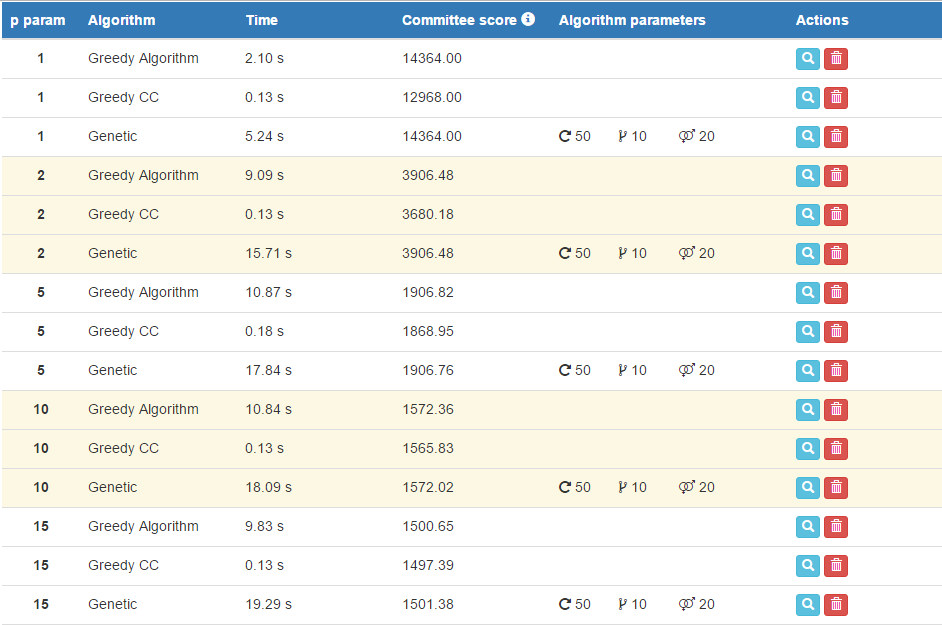
\includegraphics[scale=0.6]{pics/score_table.png}}
\captionof{figure}{Wyniki wyborów w postaci wyświetlonej przez system tabeli}
\end{center}

System wyświetla wyniki w taki sposób, aby wyniki wyborów wygenerowanych dla tego samego parametru $p$ były zgrupowane razem. W tym celu wyniki wyborów dla tego samego parametru $p$ występują obok siebie oraz mają inny kolor tła od sąsiednich wyników dla innego parametru $p$. Warto zwrócić uwagę, że w miarę wzrostu parametru $p$ wartość zadowolenia wyborców z komitetów maleje. Wynika to specyfiki funkcji satysfakcji dla systemu $\ell_p-Borda$. Porównywanie między sobą wartości zadowoleń z danego komitetu dla różnych wartości parametru $p$ raczej mija się z celem.  

\subsubsection{Prezentacja szczegółowych wyników wyborów}
Na kolejnych grafikach przedstawiono szczegółowe wyniki wyborów w postaci wykresów $2D$. Wybory wygenerowano z rozkładu
normalnego. Wyborcy i kandydaci są w nich przedstawiani jako punkty na płaszczyźnie. Wybory składają się z 30 kandydatów, 100 wyborców oraz komitetu
zwycięskiego liczącego 10 kandydatów. Wyświetlone wyniki obliczano za pomocą algorytmu
zachłannego dla rosnących parametrów $p$.
\begin{center}
\centerline{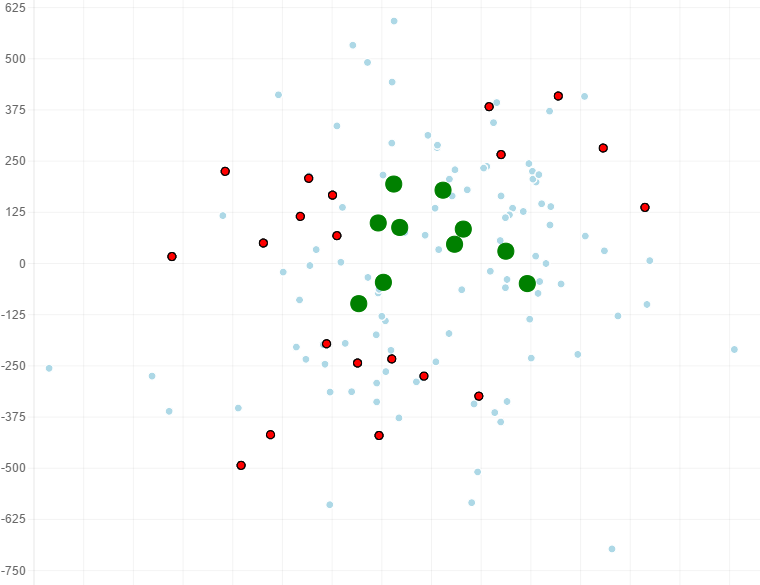
\includegraphics[scale=0.65]{pics/p1.png}}
\captionof{figure}{Wyniki wyborów dla $p$ = 1}
\clearpage
\centerline{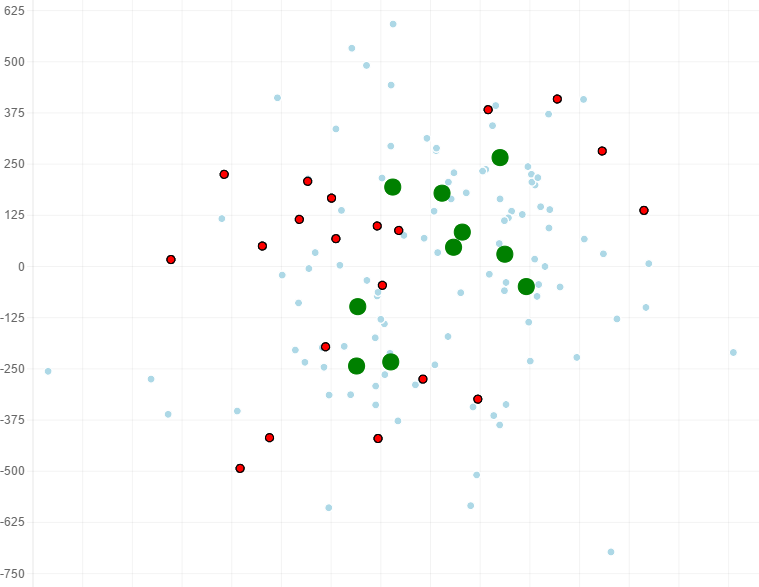
\includegraphics[scale=0.65]{pics/p5.png}}
\captionof{figure}{Wyniki wyborów dla $p$ = 5}
\centerline{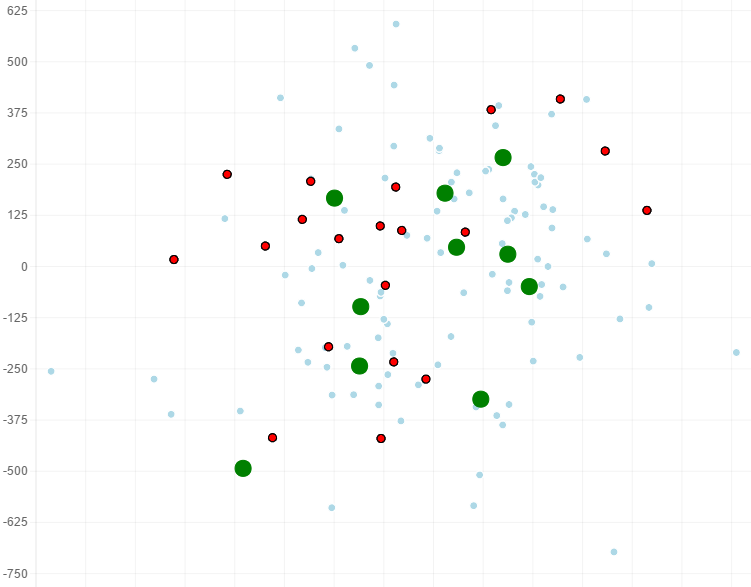
\includegraphics[scale=0.65]{pics/p20.png}}
\captionof{figure}{Wyniki wyborów dla $p$ = 20}
\end{center}

Na wykresach można zaobserwować stopniowe rozpraszanie się zwycięskich kandydatów
dla zwiększającej się wartości parametru $p$.

\section{Testy porównawcze}
\subsection{Czasy działania algorytmów}
\begin{center}
\centerline{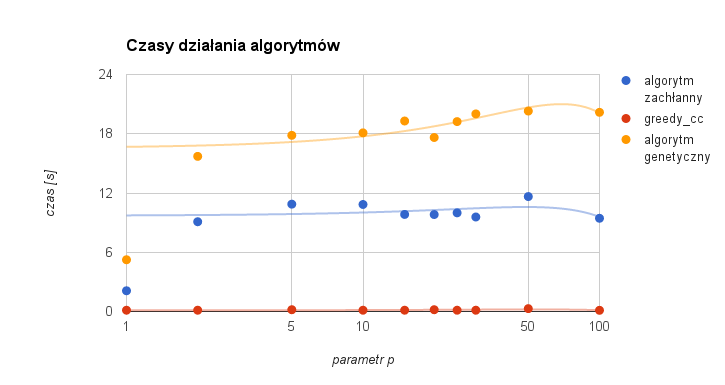
\includegraphics[scale=0.65]{pics/czas_dzialania.png}}
\captionof{figure}{Czas działania algorytmów w zależności od parametru $p$}
\end{center}
Na wykresie zaprezentowano czasy działania różnych algorytmów w zależności od
dobranego parametru $p$. Testy przeprowadzono dla wyborów zawierających $30$
kandydatów, $50$ wyborców oraz komitet zwycięski liczący $15$ kandydatów. Algorytm
zachłanny według zasady $Chamberlin-Courant’a$ nie zmienia swojego czasu obliczeń, gdyż działanie
algorytmu nie zależy od parametru $p$ . Najszybciej działa algorytm zachłanny według zasady
$Chamberlin-Courant’a$, drugi w kolejności jest algorytm zachłanny zależny od parametru $p$ , a najwolniejszy jest algorytm genetyczny.

% o ile to mozliwe prosze uzywac odwolan \cite w konkretnych miejscach a nie \nocite

%\nocite{artykul2011,ksiazka2011,narzedzie2011,projekt2011}

\bibliography{bibliografia}

\end{document}
